\section{Structure of Wikipedia}
The structure of Wikipedia is web based, where articles with similarities are linked together. Since Wikipedia is language-based, articles only link to other articles within the same language. Wikipedia does also have a category structure, where all articles are classified under at least one category. A category could have articles, but could also have subcategories, where the subcategories have their own articles and subcategories. The categories form a large category graph where articles are put under the most describing category, as an example is Ole Johan Dahl \footnote{\olejohandahleng} (Norwegian computer scientist) placed under the category \textit{Norwegian computer scientists} instead of the parent category \textit{Computer scientists by nationality}. 

The category graph is created so there is a link between a category and its subcategories. There is no beginning of the category graph, but here are some categories which have most other categories as their subcategories. These can be though of as beginning categories, often called root categories, and are important when we want to look through all categories in the graph and observe the relationships between them.  Two ategories that can be viewed as potential root categories are \textit{Fundamental Categories} and \textit{Main Topic Classifications}. If one of these are chosen as the root category, we can continue through the graph by looking at its subcategories and proceed by looking at each of the subcategory's subcategories an so on.
%An important 
%The easiest way of looking at all categories in the graph is to choose a root category and follow the links to its subcategories and then continue to look 

Figure \ref{fig: subcat_lindgren} is an example of a structure for the category \textit{Astrid Lindgren}, the swedish children's writer. The figure shows a tree structure for the category from the category graph. The figure shows that the category \textit{Astrid Lindgren} has 7 pages directly under the category, and 3 subcategories: \textit{Astrid Lindgrens karakterer} (7 pages), \textit{Astrid Lindgrens bøker} (9 pages) and \textit{Pippi Langstrømpe} (16 pages).  This means that there are indirectly 39 pages under the category \textit{Astrid Lindgren}. 


%is created and how it is fetched from the page for category information.\footnote{\categorytree}

\begin{figure}[H]
\centering
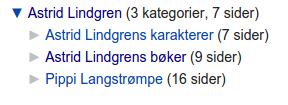
\includegraphics[height=2.5cm]{Dumps/imgs/Kategorier-Astrid-Lindgren.png}
\caption{Subcategories of the category \textit{Astrid Lindgren}. }
\label{fig: subcat_lindgren}
\end{figure}

% HVORFOR IKKE BRUKE WIKIPEDIA SINE KATEGORIER!
Articles of Wikipedia are already classified under categories, but the categorization between articles and categories cannot be used as a pre-defined category set. The reason is that articles in Wikipedia is categorize, but the categories are not guaranteed to be in the pre-defined category set. Hense it is essential that the classifier creates a connection from the article and to a category that is know to exist in the set. The classifier should instead be based on the category information provided by Wikipedia. 

%We will therefore need a mapper to a category we know exists. 
%but we cannot use either the categorization from articles to categories nor 
%this categorization is not ideal. It is not possible to use the categorization since a topic might lead
Another reason why it is not possible to use the category set in Wikipedia as the predefined category set because the category set in Wikipedia is too large. Some categories do not  provide information of the actual content, and some are too specified. There are also cases where articles are categorized under categories where the combination of the categories does not provide any new information. An example is the article of \textit{Ole Johan Dahl}. Some of the article's categories are showed in figure \ref{fig: olejohandahl_categories}. This is an example of an article where the categories provide the same information, i.e., we already know that he was from Norway since he is in the category \textit{People from Mandal, Norway}, so it would be enough to add that he was a computer scientist instead of specifying that he was a Norwegian computer scientist. 

\begin{figure}[H]
\centering
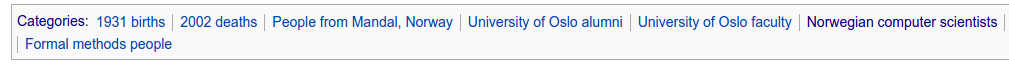
\includegraphics[width=\textwidth]{Dumps/imgs/olejohandahl-categories.png}
\caption{Some categories from the article of Ole Johan Dahl}
\label{fig: olejohandahl_categories}
\end{figure}

%set is not ideal as a predefined category set for our classifier. 
%There are two main reasons why the categories cannot be based on the categories from Wikipedia. 
%A reason for this is that an article in Wikipedia can be categorized under more than one category and these categories might not be the relevant category set. 
%In many cases are the categories directly subcategories of another category, but in some cases could it be a larger path until a common parent category and the category structure would therefore have to be flatten to make sure it is not classified under conflicting categories. 

%Hva tenkte jeg her? Another reason is that Wikipedia contains
